\documentclass{standalone}

\usepackage{tikz}
\usetikzlibrary{arrows,automata}
\usepackage[latin1]{inputenc}
\begin{document}
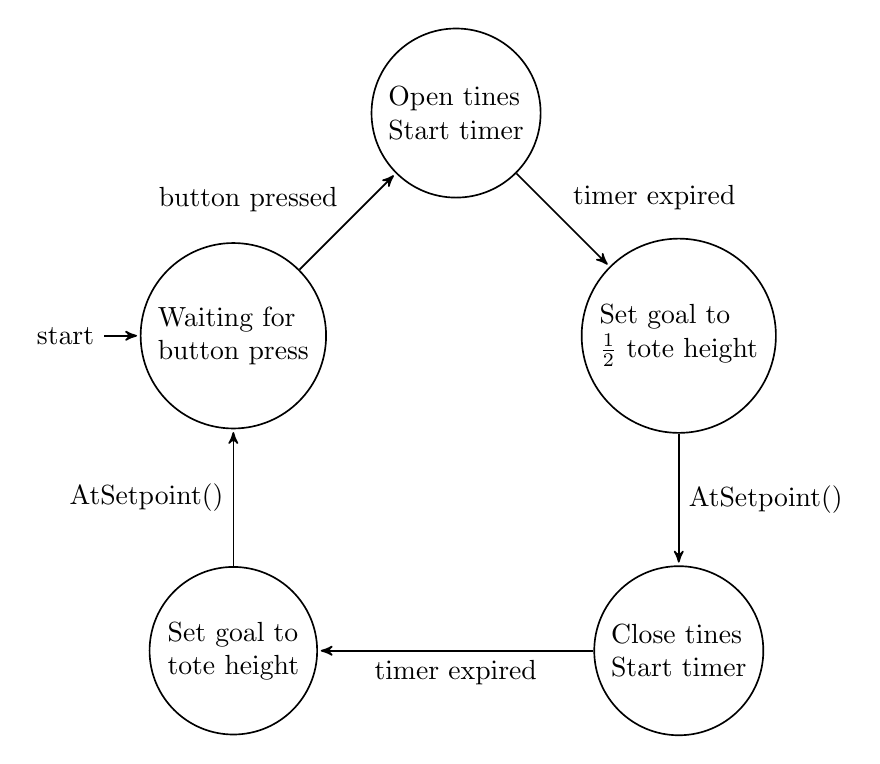
\begin{tikzpicture}[->,>=stealth',shorten >=1pt,auto,node distance=4cm,
                    semithick]
  \tikzstyle{every state}=[fill=white,draw=black,text=black]

  \node[initial,state] (A) [align=left] {Waiting for\\button press};
  \node[state] (B) [above right of=A,align=left] {Open tines\\Start timer};
  \node[state] (C) [below right of=B,align=left]
    {Set goal to\\$\frac{1}{2}$ tote height};
  \node[state] (D) [below of=C,align=left] {Close tines\\Start timer};
  \node[state] (E) [below of=A,align=left] {Set goal to\\tote height};

  \path (A) edge node {button pressed} (B)
        (B) edge node {timer expired} (C)
        (C) edge node {AtSetpoint()} (D)
        (D) edge node {timer expired} (E)
        (E) edge node {AtSetpoint()} (A);
\end{tikzpicture}
\end{document}
